\section{Introduci\'on}
	\subsection{El modelo OSI y la arquitectura TCP/IP}
		\setlength{\parindent}{1em}
		\setlength{\parskip}{10pt}
			El modelo OSI nace de la necesidad de tener un est\'andar para la comunicaci\'on en redes amplias o sea equipos de distintos fabricantes, as\'i como facilitar econom\'ias a gran escala y debido a la complejidad que implican estas comunicaciones de proporciones b\'iblicas, por ello las distintas funcionalidades se dividen en partes mas manejables, por ello el modelo OSI fue muy aceptada para estructurar problemas, y fue adoptada por el ISO. En esta t\'ecnica, las funciones de comunicaci\'on se distribuyen en un conjunto jer\'arquico de capas. Cada capa realiza un subconjunto de tareas relacionadas entre s\'i, de entre las necesarias para llegar a comunicarse con otros sistemas. Por otra parte, cada capa se sustenta en la capa inmediatamente inferior, la cual realizar\'a funciones m\'as primitivas, ocultando los detalles a las capas superiores. Una capa proporciona servicios a la capa inmediatamente superior. Idealmente, las capas deber\'ian estar definidas para que los cambios en una capa no implicaran cambios en las otras capas. De esta forma, el problema se descompone en varios subproblemas m\'as abordables.
\vskip 1pt
La arquitectura de protocolos TCP/IP es resultado de la investigaci\'on y desarrollo llevados a cabo en la red experimental de conmutaci\'on de paquetes ARPANET, financiada por la Agencia de Proyectos de Investigaci\'on Avanzada para la Defensa (DARPA, Defense Advanced Research Projects Agency), y se denomina globalmente como la familia de protocolos TCP/IP. Esta familia consiste en una extensa colecci\'on de protocolos que se han especificado como est\'andares de Internet por parte de IAB (Internet Architecture Board).
\begin{figure}[h]
			\centering		
			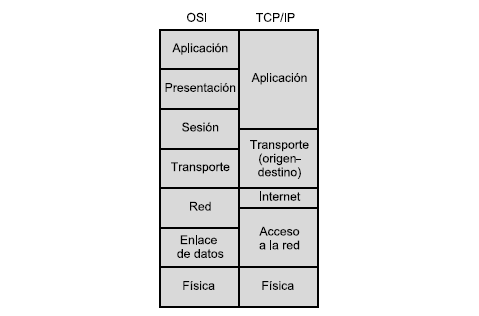
\includegraphics[width=\textwidth]{OSITCP}
			\caption{Comparaci\'on entre las arquitecturas de protocolos TCP/IP y OSI.}
		\end{figure}
		\clearpage
		\subsubsection{Encapsulado del modelo OSI}
			Veremos cual es el proceso de encapsulamiento del modelo OSI:
		\vskip 1pt
		CAPA 7. La informaci\'on comienza con el nombre de datos en la Capa de Aplicaci\'on en el lado del emisor
		\vskip 0.25pt
		CAPA 6. Conforme los datos se mueven a la Capa de Presentaci\'on es codificado o comprimido a un formato est\'andar a veces encriptado. Despu\'es los datos del usuario son convertidos a un formato est\'andar com\'un
	\vskip 0.25pt
		CAPA 5. Despu\'es se mueve a la Capa de Sesi\'on. En esta capa, un ID de sesi\'on se agrega a los datos. (Hasta este punto los datos todav\'ia tienen su estructura original)
		\vskip 0.25pt
		CAPA 4. Ahora los datos pasan a la Capa de Transporte en la capa de transporte los datos son fraccionados en diferentes y m\'as peque\~nos bloques o piezas. A cada bloque se le agrega una cabecera, que contiene:
		\begin{enumerate}
			\item Puertos de destino y Origen 
			\item N\'umeros de secuencia y otra informaci\'on 
			\item Todos en conjunto crean un nuevo PDU
			\item El nuevo PDU se llama Segmento si TCP es el protocolo utilizado, o lo llamaremos Datagrama si se trata de UDP.
		\end{enumerate}
		\vskip 0.25pt
		CAPA 3. Cuando el segmento viaja a la Capa de Red una nueva cabevera de IP se agrega. Esta cabecera de IP contiene la direcci\'on IP origen y la direccion IP destino y otra informaci\'on
\vskip 0.25pt
		CAPA 2. Cuando el paquete pasa a Capa de Enlace; se repite el proceso y se agrega una cabecera y un bloque llamadao FCS al final del paquete en esta capa un nuevo PDU llamado frame o trama es creado. La cabecera de la trama contiene  la direcci\'on MAC de origen y destino y como otro control de informaci\'on. FCS marca el final de la trama y tambi\'en se usa para verificar
\vskip 0.25pt
		CAPA 1. El frame ahora es enviado a la Capa f\'isica. En esta capa f\'isica solo se consideran los 1 y 0's que representan a la trama es por eso que a este tipo de PDU normalmente se le llaman los Bits. Los 1 y 0's entonces est\'an listos para ser convertidos en cualquier tipo de se\~nal ya sea electrica, ondas de radio, luz, etc.
\vskip 1pt
		Ahora realizaremos el proceso de desencapsulamiento: 
\vskip 0.25pt
		 CAPA 1 y CAPA 2.- La Capa F\'isica recibe bits y los manda a la Capa de Enlace de datos donde son interpretados como una trama y se
Verifica su cabercera e informaci\'on adicional a\~nadida, si la MAC address tiene correspondencia y no se encuentran errores entronces la trama es descartada y el paquete IP extraido y entregado a la capa de red.

CAPA 3.- En la Capa de Red la cabecera IP es verificada y si esta IP concuerda entonces la cabercera IP es eliminada del paquete IP.

CAPA 4.- Ahora el segmento pasa a la Capa de Transporte donde se examina esta informaci\'on, se busca el numero de puerto.

CAPA 5.- La informaci\'on es transferida a la Capa de Sesi\'on considerando la aplicaci\'on que le corresponde Seg\'un el numero de puerto. En este punto un ID de sesi\'on se ocupa.

CAPA 6 Y 7.- Los datos pasan ahora a la Capa de Presentaci\'on cualquier encriptado ser\'a removido y el datos ser\'a recuperado a su forma original que entonces ser\'a presentada a la Capa de Aplicaci\'on.
		\begin{figure}[h]
			\centering		
			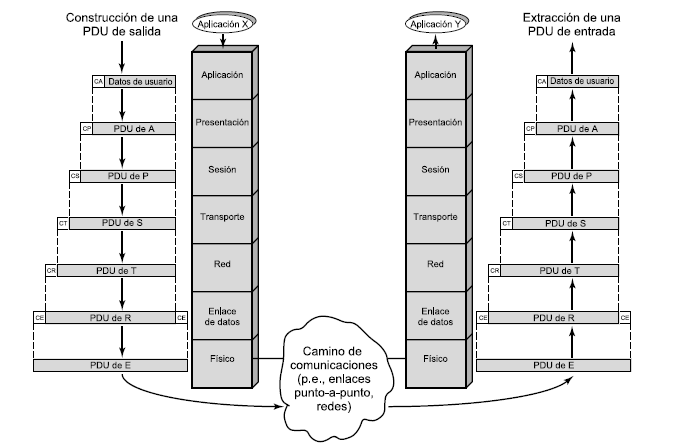
\includegraphics[width=\textwidth]{EntornoOSI}
			\caption{El entorno OSI}
		\end{figure}
		\clearpage
		\subsection{Cabecera Ethernet}
		Para poder hablar propiamente de la cabecera ethernet, tenemos que hablar de las cabeceras de paquete de interfaz de red.
\vskip 1pt
		En esta capa de iterfaz de red, se adjuntan cabeceras de paquete a los datos de salida, los paquetes se tienen que enviar a tr\'aves del adaptador de red a la red apropiada. Los paquetes pasan por muchas pasarelas antes de alcanzar los destinos. En la red de destino, las cabeceras se separan de los paquetes y se env\'ian los datos al sistema principal apropiado.
\vskip 1pt
		Pasando al tema principal que ser\'ia la cabecera ethernet, esta esta compuesta simplemente por 14 bytes, en donde los primeros 6 bytes es la direcci\'on destino, los siguientes 6 bytes es la direcci\'on origen y los 2 restantes es el tama\~no o tipo, si es menor a 1500 es tama\~no y nos da el mismo de la cabecera LLC, si es 0800 y 0806 en hexadecimal son IP y ARP respectivamente.
	\begin{figure}[h]
			\centering		
			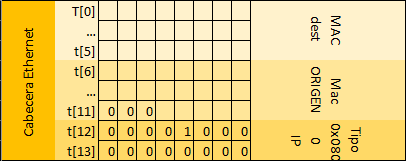
\includegraphics[width=\textwidth]{MapaMemoriaCEthernet}
			\caption{El mapa de memoria para la cabecera Ethernet}
		\end{figure}
		\begin{lstlisting}[language={C}, caption={Funcion que Analiza Cabecera Ethernet}, label={Script}]
	void leerTrama(unsigned char * T){
    printf("\nCabecera ethernet \n");
    unsigned short tot = T[12] << 8 | T[13];
    printf("MAC DESTINO %.2x: %.2x: %.2x: %.2x: %.2x: %.2x\n", T[0], T[1], T[2], T[3], T[4], T[5]);
    printf("MAC ORIGEN %.2x: %.2x: %.2x: %.2x: %.2x: %.2x\n", T[6], T[7], T[8], T[9], T[10], T[11]);
    if (tot < 1500){
        printf("Tamano de la cabecera LLC: %d bytes \n", tot);
        analizarTrama(T);
    }else{
        if (tot == 2048){
            printf("TIPO IP\n");// analiza IP
        }else if (tot == 2054){
            printf("TIPO ARP\n");// analiza ARP
            analizaARP(T);
        }else{
            printf("TIPO: %.2x%.2x", T[12], T[13]);
        }
    }
}
	\end{lstlisting}
		\clearpage
	\subsection{El Protocolo IP(Internet Protocol)}
		El protocolo IP es el encargado de transmitir datagramas desde un host a otro, si fuera necesario, via routers intermediarios. IP proporciona un servicio de entrega que se puede describir como no fiable o el mejor posible, best-effort, porque no existe garantia de entrega. Los paquetes se pueden perder, ser duplicados, sufrir retrasos o ser entregados en un orden distinto al original, pero esos errores solo ocurren cuando los buffers en el destino est\'an llenos. La \'unica comprobaci\'on de errores realizada por IP es el checksum, de la cabecera, que es asequible de calcular y asegura que no se han detectado alteraciones en los datos bien de direccionamiento o bien de gesti\'on de paquete.
	\begin{figure}[h]
			\centering		
			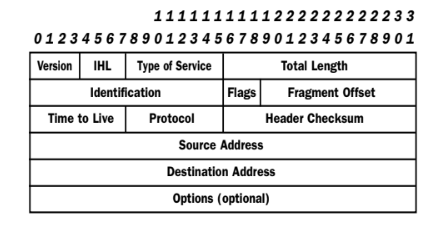
\includegraphics[width=\textwidth]{CabeceraIP}
			\caption{Son los campos de la cabecera IP}
		\end{figure}
\vskip 1pt
En los campos primeramente tenemos al de version, este campo nos sirve para la version del protocolo IP, ya sea IPv4 o IPv6; el segundo campo, el IHL nos sirve para obtener el tama\~no de nuestra cabecera IP, que puede ser de 20 a 60 bytes (el tama\~no total de mi cabecera IP), basicamente es para el campo llamado opciones si el campo es 5, es que no tiene opciones, el siguiente campo nos sirve para el tipo de servicio que es, ya sea uno de costo minimo, fiabilidad maxima, etc; despues nos da el numero de bytes en el paquete, el tama\~no maximo es de 65 535 bytes, despues tenemos al identificador, que nos dice que valor de ID tiene; despues tenemos las banderas, que tiene 3 valores, x(reservado), D = 1(dont fragment), y M = 1(More Fragment), despu\'es tenemos el Fragment offset en el que tenemos que posicionarlo en el datagrama original; despu\'es tenemos el time to live que nos dice el tiempo de vida de nuestro protocolo; despu\'es tenemos lo que seria nuetro protocolo que usaremos despues, que en nuestro caso usaremos solo ICMP, TCP y UDP; ahora tenemos el checksum que mas arriba explicamos para que sirve; y solo nos quedan las direcciones IP de destino y origen junto con las Opciones si es que tiene.
\vskip 1pt
El tama\~no maximo de la cabecera IP es de 60 bytes, el tama\~no minimo de la cabecera es de 20 bytes, y el tama\~no maximo del IHL es de 15, el tama\~no minimo del es de 5.
		\begin{figure}[h]
			\centering		
			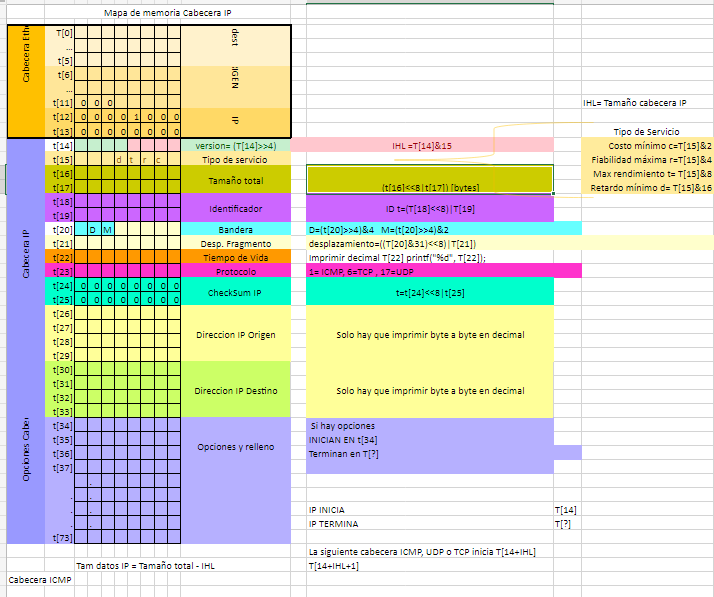
\includegraphics[width=\textwidth]{MapaMemoria}
			\caption{Es el mapa de memoria de la cabecera IP}
		\end{figure}